\documentclass{article}

%% Page Margins %%
\usepackage{geometry}
\geometry{
    top = 0.75in,
    bottom = 0.75in,
    right = 0.75in,
    left = 0.75in,
}

\usepackage{amsmath}
\usepackage{graphicx}
\usepackage{parskip}

\title{Lab 4: Synchronous Sequential Circuits}

% TODO: Enter your name
\author{Qianjun Huang}

\begin{document}
\maketitle

\section*{Part Ia}

\begin{enumerate}
\setcounter{enumi}{1}
\item Export the subcircuit schematic as an image and include it in your report.

\begin{figure}[ht!]
    \centering
    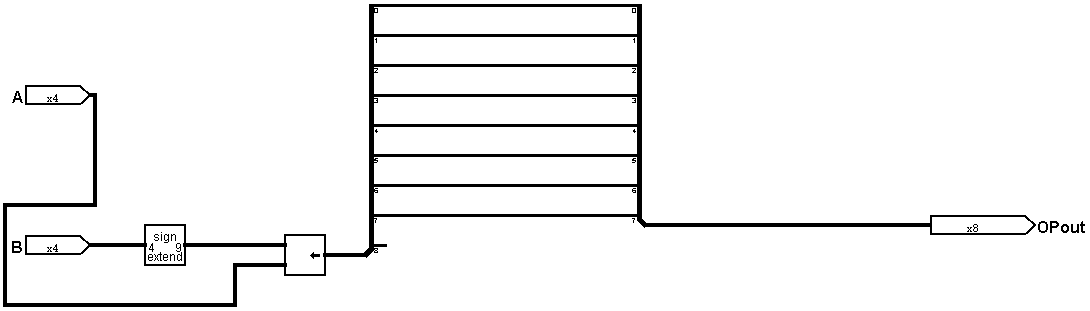
\includegraphics[width=0.4\textwidth]{lab4_op5.png}
    \caption{A schematic of op5.}
    \label{f:op5}
\end{figure}

\begin{figure}[ht!]
    \centering
    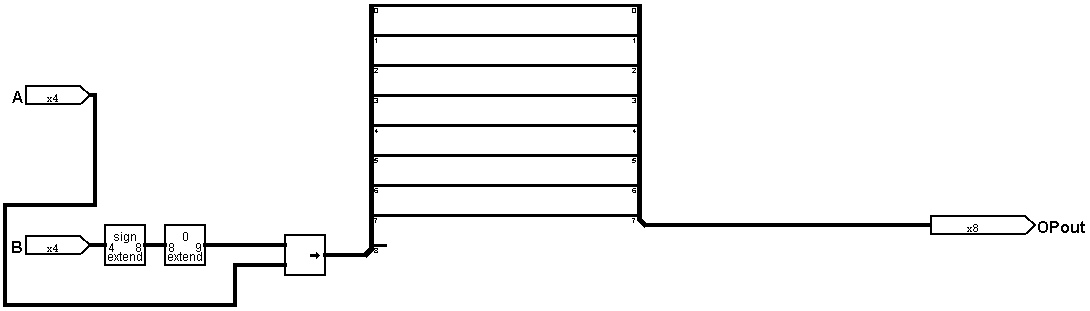
\includegraphics[width=0.4\textwidth]{lab4_op6.png}
    \caption{A schematic of op6.}
    \label{f:op6}
\end{figure}

\begin{figure}[ht!]
    \centering
    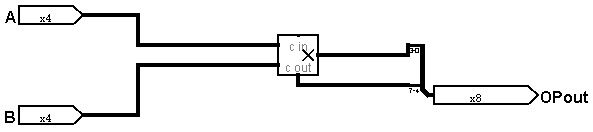
\includegraphics[width=0.4\textwidth]{lab4_op7.png}
    \caption{A schematic of op7.}
    \label{f:op7}
\end{figure}

\item Include a screenshot of your simulated test vectors for op5, op6, and op7.

\begin{figure}[ht!]
    \centering
    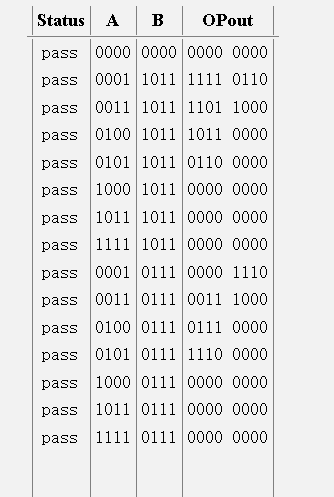
\includegraphics[width=0.4\textwidth]{lab4_op5_simulation.png}
    \caption{A simulation of op5.}
    \label{f:op5_simulation}
\end{figure}

\begin{figure}[ht!]
    \centering
    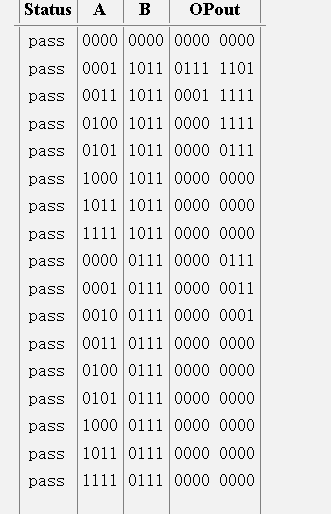
\includegraphics[width=0.4\textwidth]{lab4_op6_simulation.png}
    \caption{A simulation of op6.}
    \label{f:op6_simulation}
\end{figure}

\begin{figure}[ht!]
    \centering
    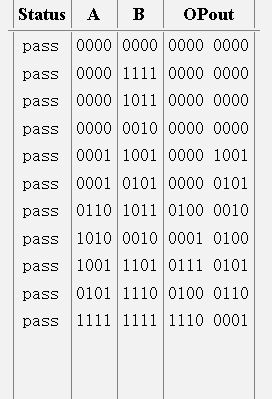
\includegraphics[width=0.4\textwidth]{lab4_op7_simulation.png}
    \caption{A simulation of op7.}
    \label{f:op7_simulation}
\end{figure}


\end{enumerate}

\section*{Part Ib}

\begin{enumerate}
\setcounter{enumi}{2}
\item Include a screenshot of your simulated timing diagram demonstrating ALUreg starting at 0x0 and increasing by 1 until 0x0f.

\begin{figure}[ht!]
    \centering
    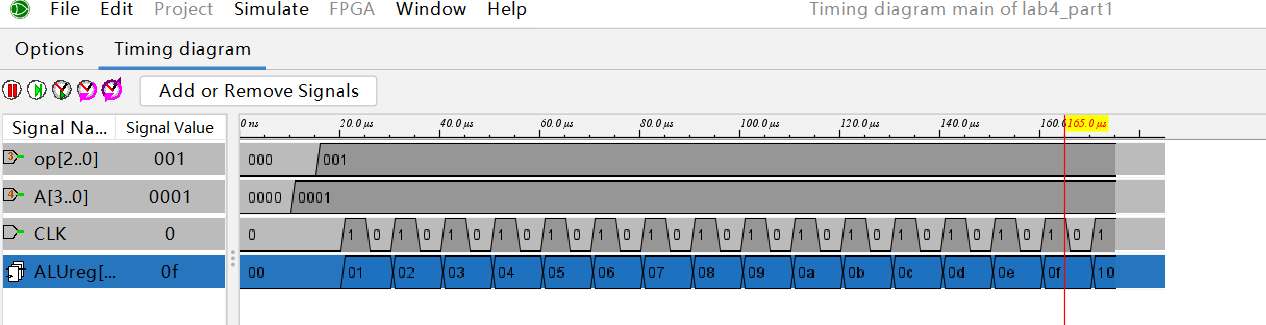
\includegraphics[width=0.4\textwidth]{lab4_timing_plus_one.png}
    \caption{A timing simulation demonstrating incrementing.}
    \label{f:timing_plus_one}
\end{figure}

\item Include a screenshot of your simulated timing diagram demonstrating a shifting operation where ALUreg goes from at 0x01 and doubling until 0x00.

\begin{figure}[ht!]
    \centering
    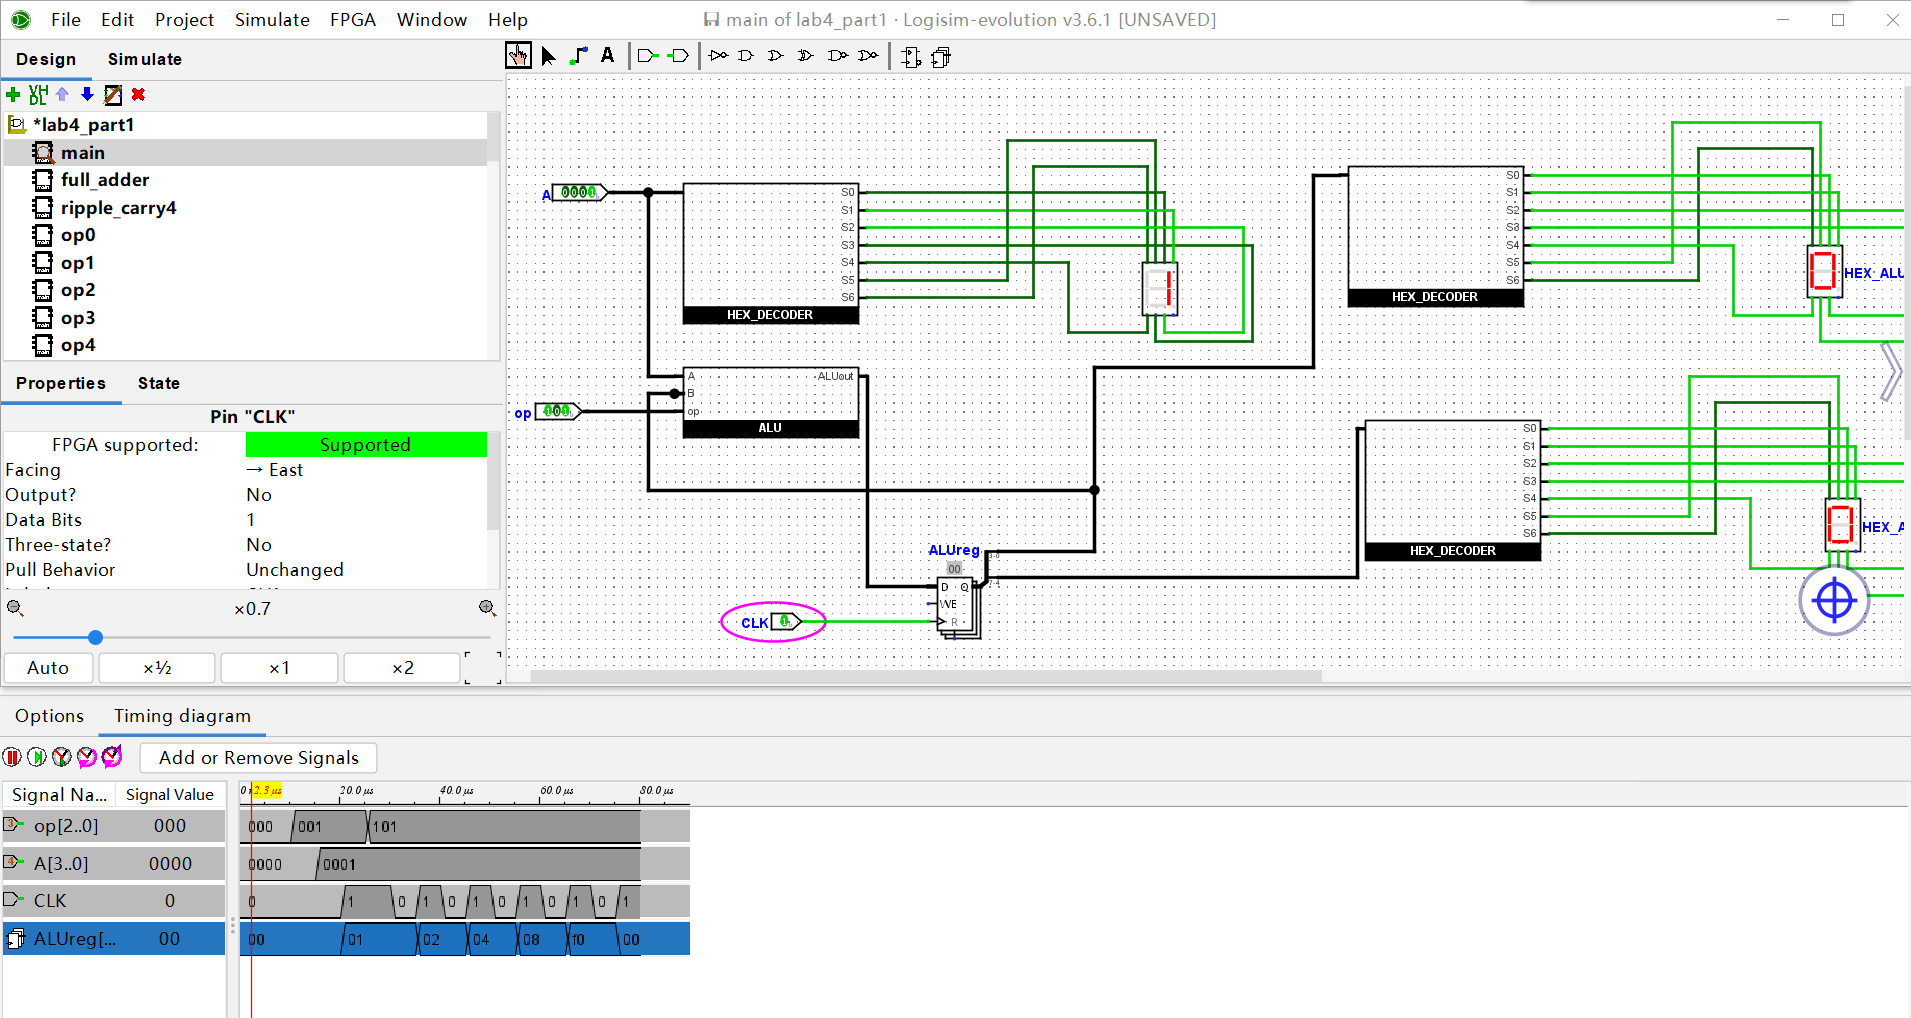
\includegraphics[width=0.4\textwidth]{lab4_timing_times_two.png}
    \caption{A timing simulation demonstrating doubling.}
    \label{f:timing_double}
\end{figure}
\end{enumerate}

\section*{Part II}

\begin{enumerate}
\setcounter{enumi}{1}
\item Export the subcircuit schematic as an image and include it in your report.

\begin{figure}[ht!]
    \centering
    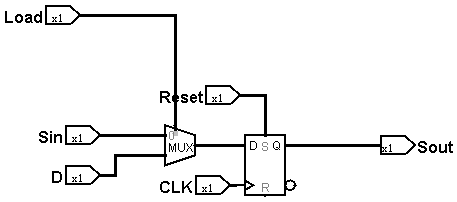
\includegraphics[width=0.5\textwidth]{lab4_shifter_bit.png}
    \caption{A schematic of the shifter\_bit.}
    \label{f:shifter_bit}
\end{figure}

\item Include a screenshot of your simulated timing diagram demonstrating that the output can take on values from either input.

\begin{figure}[ht!]
    \centering
    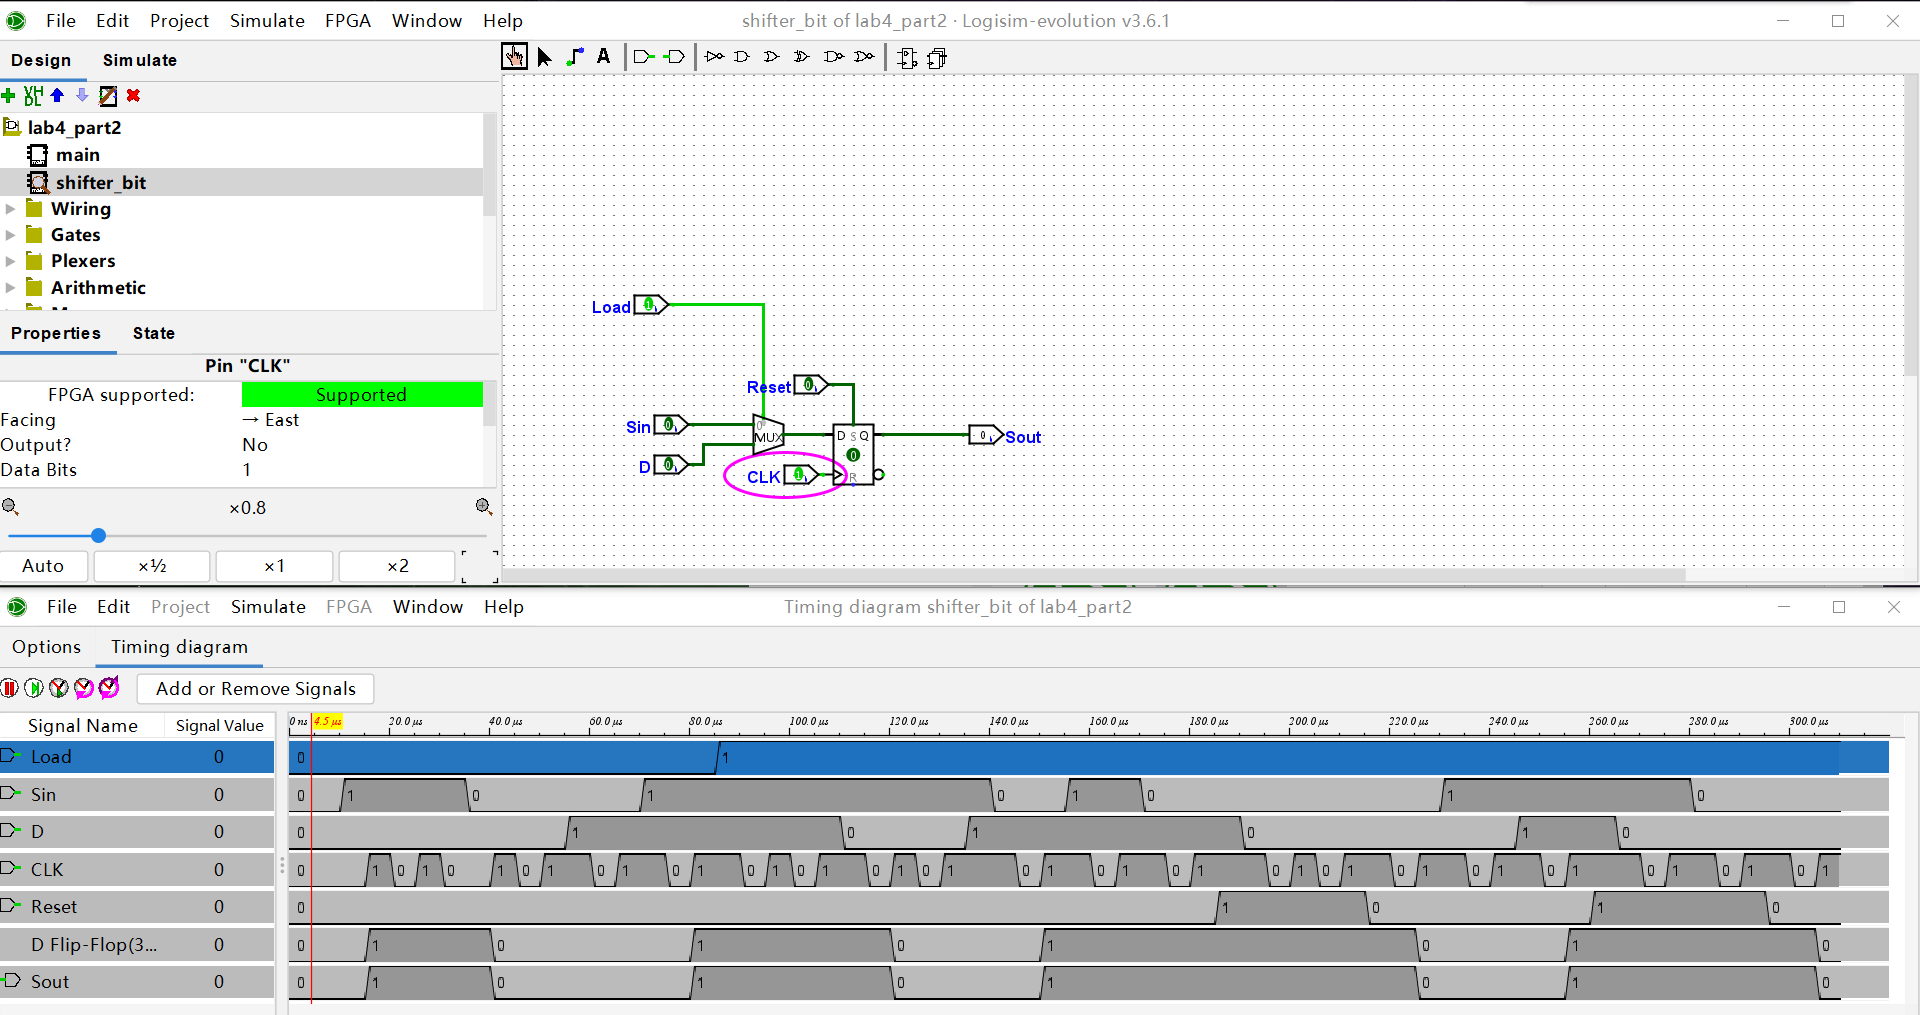
\includegraphics[width=0.5\textwidth]{lab4_timing_shifter_bit.png}
    \caption{A timing simulation of the shifter\_bit.}
    \label{f:timing_shifter_bit}
\end{figure}
\end{enumerate}

\end{document}